\documentclass[a0,portrait]{a0poster}

%\usepackage[portuguese]{babel}%Formata as entradas para PT-BR
%\usepackage[utf8]{inputenc}
%\usepackage{verbatim}
\usepackage[document]{ragged2e}
\usepackage{multicol} % This is so we can have multiple columns of text side-by-side
\columnsep=90pt % This is the amount of white space between the columns in the poster
\columnseprule=0pt % This is the thickness of the black line between the columns in the poster

\usepackage[svgnames]{xcolor} % Specify colors by their 'svgnames', for a full list of all colors available see here: http://www.latextemplates.com/svgnames-colors

\usepackage{times} % Use the times font
%\usepackage{palatino} % Uncomment to use the Palatino font
%\usepackage{varioref}
%\usepackage{hyperref}
%\usepackage{epsfig}
\usepackage{graphicx} % Required for including images
\graphicspath{{figures/}} % Location of the graphics files
\usepackage{booktabs} % Top and bottom rules for table
\usepackage[font=small,labelfont=bf]{caption} % Required for specifying captions to tables and figures
\usepackage{amsfonts, amsmath, amsthm, amssymb} % For math fonts, symbols and environments
\usepackage{mathrsfs}
\usepackage{wrapfig} % Allows wrapping text around tables and figures
\usepackage{setspace}
\usepackage{xcolor}
\usepackage[left=3cm, top=2cm, right=3cm, bottom=0cm]{geometry}
\usepackage{enumitem}
\usepackage{blindtext}
\setitemize{labelsep=1cm,leftmargin=*}
\usepackage{vwcol}

\begin{document}
\onehalfspacing
%----------------------------------------------------------------------------------------
%	POSTER HEADER 
%----------------------------------------------------------------------------------------

% The header is divided into two boxes:
% The first is 75% wide and houses the title, subtitle, names, university/organization and contact information
% The second is 25% wide and houses a logo for your university/organization or a photo of you
% The widths of these boxes can be easily edited to accommodate your content as you see fit

\vspace{50cm}

\begin{table}[ttt]
\begin{center}
%\vspace*{-2cm}
\vspace{1.5cm}
\begin{tabular}{lcr}
\begin{tabular}{c} \vspace{-2cm} \\ 
\includegraphics[scale=1]{ita.jpg} \end{tabular} & \hspace{1cm} \begin{tabular}{c} \vspace*{-0cm} \LARGE{20$^{\textrm{th}}$ Brazilian Workshop on Semiconductor Physics - BWSP} \\ \LARGE{Aeronautics Institute of Technology - ITA, Brazil} \\ \vspace{0.5cm} \LARGE{National Council for
Scientific and Technological Development - CNPq}
\end{tabular} & \hspace{1cm} \begin{tabular}{r} \vspace{-1cm} \\ 
\includegraphics[scale=1.2]{BWSPlogo.png} \end{tabular}
\end{tabular}
\end{center}
\end{table}

\vspace{30cm}

\begin{minipage}[b]{1.0\linewidth} %default 0.75
\begin{center}

\vspace{1cm}
\Huge \textbf{PHYSICAL PROPERTIES OF INTERFACES BETWEEN TiO$_2$ AND PEROVSKITES WITH QUASIPARTICLE DFT-1/2 CORRECTION}\\


\LARGE \textbf{Vinicius Gabriel$^{1}$, Ivan Guilhon$^{2}$, Lara K. Teles$^{2}$ and Marcelo Marques$^{2}$}\\

\normalsize $^1$Engineering School of Lorena - University of São Paulo, SP, Brazil\\
\normalsize $^2$Semiconductor Materials and Nanotechnology Group - Aeronautics Institute of Technology, SP, Brazil\\[0.1cm]

\end{center}
\end{minipage}
%
\vspace{0.5cm} % A bit of extra whitespace between the header and poster content

%----------------------------------------------------------------------------------------
\vspace{-2.5cm}


\vspace{1cm}


\begin{multicols}{3}

\justify % Justify all text

\Large


\hrulefill
\vspace{-0.7cm}
\begin{center} 
\Large \bf{INTRODUCTION AND GOAL}
\end{center}
\vspace{-1.5cm}
\hrulefill

\begin{itemize}
%\item Fast increase of PCE and relatively easy processing methods for perovskite solar cells.

%\item Physical properties of the interfaces within the device play a crucial role for the stability and efficiency of the cell.
\item Interfaces between layers play a crucial role for efficiency of the solar cell.
\item We aim to study theoretically interfacial properties by means of the explicit heterostructure using DFT-1/2 [1, 2].
\end{itemize}

\vspace{1.5cm}

\begin{center}
\begin{tabular}{c}
\includegraphics[scale=0.4]{nanoestruturas.png} \\
\end{tabular}
\end{center}
\vspace{-1cm}
\captionof{figure}{Perovskite (ABX$_3$) and TiO$_2$ nanostructures}
\vspace{1cm}


\hrulefill
\vspace{-0.8cm}
\begin{center} 
\Large \bf{METHODOLOGY}
\end{center}
\vspace{-1.5cm}
\hrulefill


\begin{itemize}
\item All calculations runned on VASP code [3].
\item Removal of half electron from the most predominant orbital in the valence band for DFT-1/2 implementation using the software minushalf [4].
\item Heterostructure with 22 atomic layers and 405 atoms in total.
\item Projected density of states in each atomic layer.
\\
\\
\\
\end{itemize}

%\begin{center}
%\begin{tabular}{c}
%
\includegraphics[scale=0.9]{vasp.png} \\
%\end{tabular}
%\end{center}
%\vspace{-1cm}
%\captionof{figure}{VASP Code logo [4]}
%\vspace{1cm}

\hrulefill
\vspace{-0.7cm}
\begin{center} 
\Large \bf{CONCLUSIONS}
\end{center}
\vspace{-1.5cm}
\hrulefill

\begin{itemize}
\item The quasiparticle correction DFT-1/2 and SOC implementation provided accurated values for the compounds properties.
%\item The perovskites compounds studied undergo a large strain when are above the oxide.
\item This method provides a rigorous description of real interfaces, going beyond the simplified models presented in the literature.
\item With quasiparticle correction, the band alignment tends to approximate from type 2, but it is required SOC effect employment for further description.
\item It is necessary a longer heterostructure to achieve bulk properties.
\end{itemize}


\end{multicols}

\vspace{1cm}

\hrulefill
\vspace{-0.7cm}
\begin{center} 
\Large \bf{RESULTS AND DISCUSSIONS}
\end{center}
\vspace{-0.8cm}
\hrulefill


\begin{multicols}{2}

\begin{center}
\begin{tabular}{c}
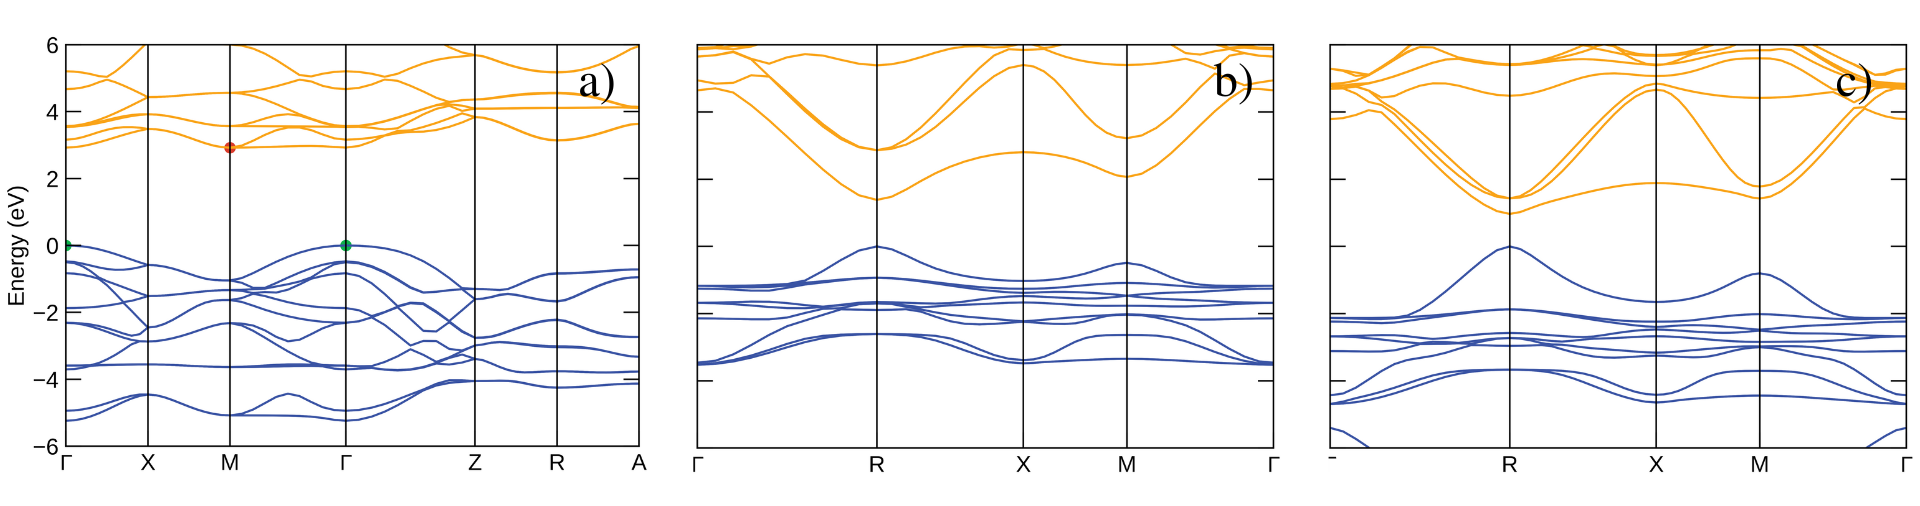
\includegraphics[scale=0.72]{allbands.png} \\
\end{tabular}
\end{center}
\vspace{-1cm}
\captionof{figure}{Band structure of (a) TiO$_2$, (b) CsPbI$_3$ and (c) CsSnI$_3$}
\vspace{1cm}

\begin{center}
\begin{tabular*}{\columnwidth}{@{\extracolsep{\fill}}cccccccccc}
%\centering
\toprule
 & \multicolumn{4}{c}{lattice parameter (\AA)} & \multicolumn{5}{c}{bandgap (eV)} \\
\midrule
Compound & a & c & (s)a & (s)c & DFT & DFT-1/2 & SOC + DFT-1/2 & Exptl & (s) SOC + DFT-1/2 \\
\midrule
TiO$_2$ & 4.670 & 2.967 & - & - & 1.717 & 2.924 & 2.924 & 3.051 [5] & -\\
CsPbI$_3$ & 6.388 & 6.388 & 7.005 & 6.242 & 1.472 & 2.545 & 1.385 & 1.68 [6] & 1.612 \\
CsSnI$_3$ & 6.270 & 6.270 & 7.005 & 6.108 & 0.450 & 1.348 & 0.967 & 1.27 [7] & 1.523 \\
\bottomrule
\end{tabular*}
\captionof{table}{Lattice parameter (\AA) and bandgap (eV) of the bulk and bulk strained (s) for cubic and tetragonal structures}
\end{center}


\vspace{0.2cm}


\begin{center}
\begin{tabular}{c}
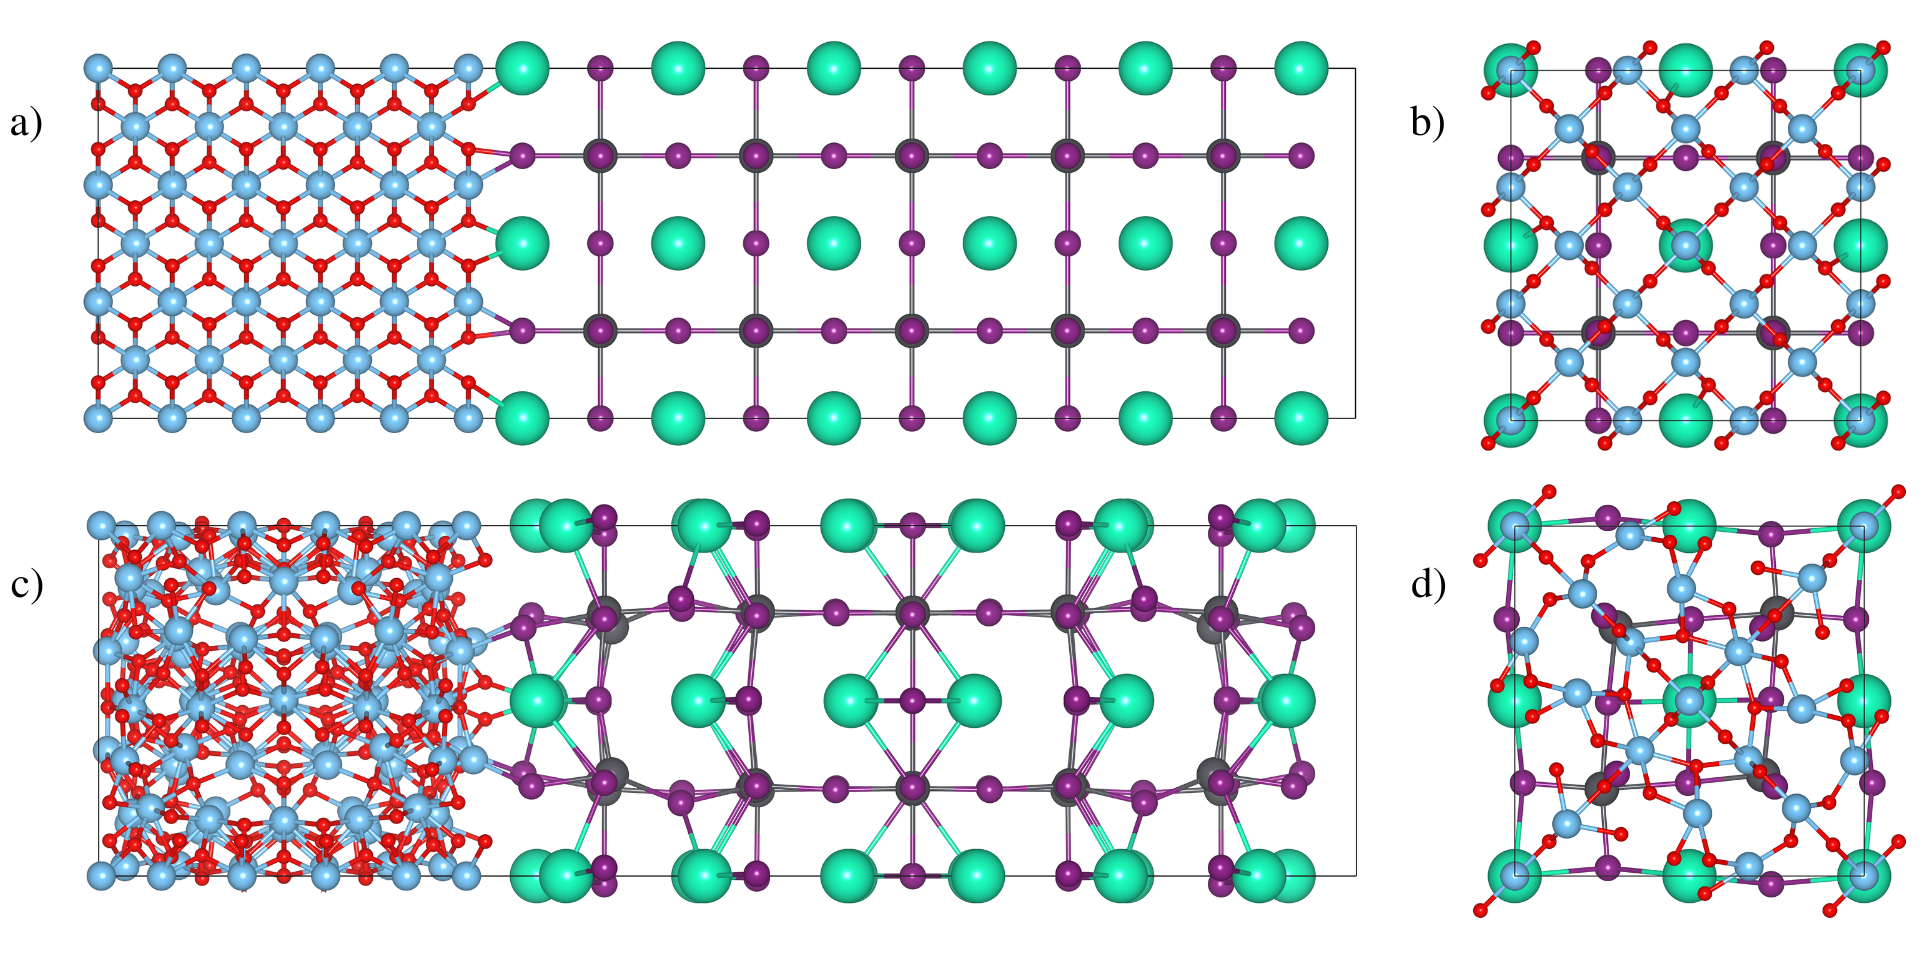
\includegraphics[scale=0.725]{interfacerelaxationwsurface.png} \\
\end{tabular}
\end{center}
\vspace{-1cm}
\captionof{figure}{Heterostructure (a) non-relaxed, (b) the 4 layers of contact, (c) heterostructure relaxed and (d) its 4 layers of contact}
\vspace{1cm}

\begin{center}
\begin{tabular}{c}
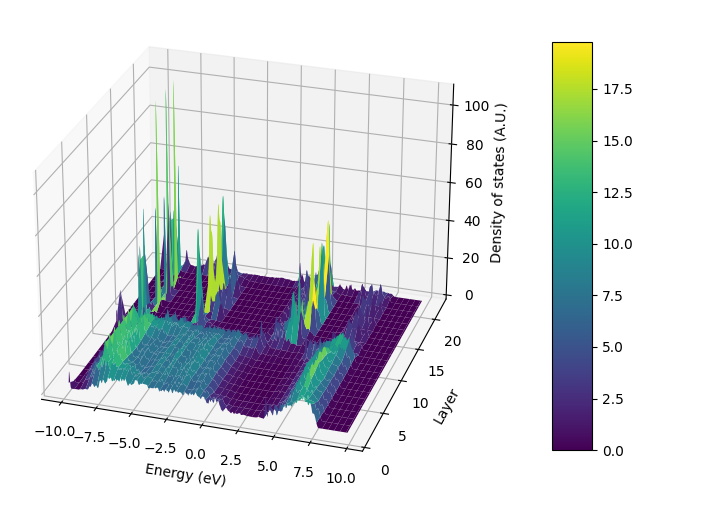
\includegraphics[scale=1.7]{pdosviridis.png} \\
\end{tabular}
\end{center}
\vspace{-1cm}
\captionof{figure}{Projected density of states in each layer}
\vspace{1cm}

\begin{center}
\begin{tabular}{c}
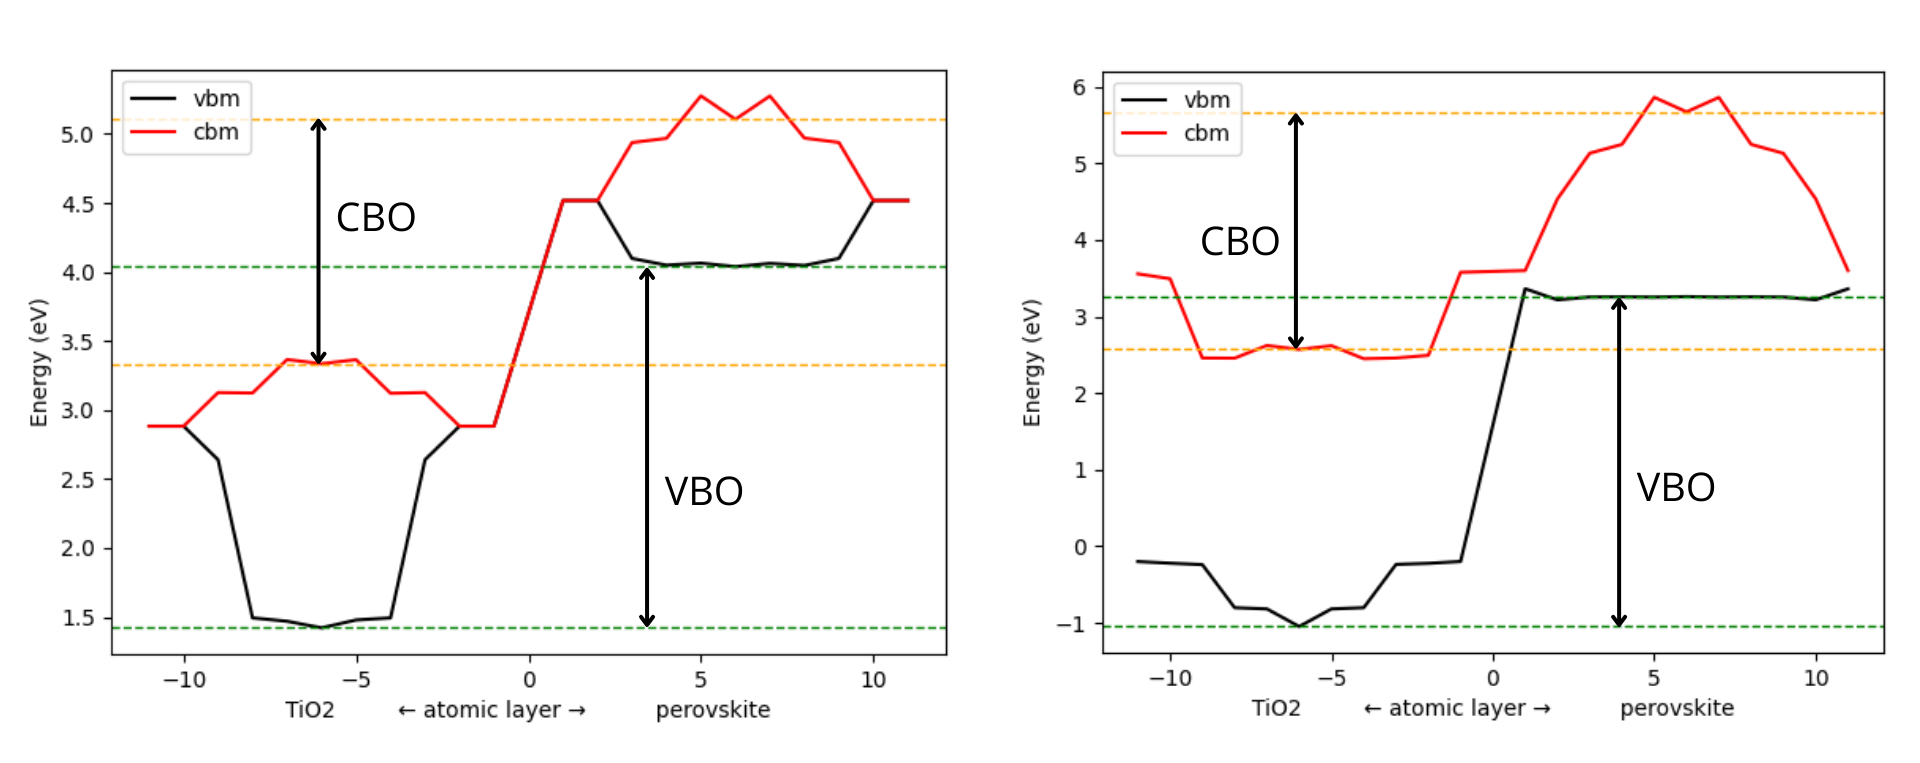
\includegraphics[scale=0.7]{offsets.png} \\
\end{tabular}
\end{center}
\vspace{-1cm}
\captionof{figure}{Band alignment for TiO$_2$ - CsPbI$_3$ heterostructure using DFT (left) and DFT-1/2 (right)}
\vspace{1cm}

\end{multicols}


\vspace{1cm}
\nocite{*} % Print all references regardless of whether they were cited in the poster or not


\begin{table}[hhh]
\begin{tabular}{cr}

\hspace{2cm}

\begin{tabular}{c}
\begin{tabular}{lcccccc}
\toprule 
 & VBO & CBO & bandgap (TiO$_2$) & aim & bandgap (CsPbI$_3$) & aim \\
\midrule 
DFT & 2.617 & 1.771 & 1.914 & 1.717 & 1.213 & 1.518 \\
DFT-1/2 & 4.306 & 3.101 & 3.617 & 2.924 & 2.412 & 2.768 \\
\bottomrule
\end{tabular}
\\
\vspace{0cm}
\\

\small{\textbf{Table 2:} Valence (VBO) and conduction (CBO) band offset and bandgap in the middle of each side, all in eV}

\\
\vspace{0.5cm}

\begin{minipage}{30cm}
\justify
\
\begin{itemize}
\item{\large Previously works provide average values of 2.285 eV and 0.637 eV \\[0.3cm] for VBO and CBO [8-10], all values with respect to the vacuum level.\\[0.3cm]However, there is a lack of works that calculate the energy alignment\\[0.3cm] for the heterostructure. This is what we desire obtain.}
\end{itemize}
\end{minipage}

\end{tabular}

&

\hspace{7cm}

\begin{minipage}{35cm}

\Large{\bf References}

\scriptsize{
\begin{itemize}[labelindent=1em]
%\bibitem{-051}
\item[{[1]}]FERREIRA, L. G.; MARQUES, M.; TELES, L. K. Approximation to density functional theory for the calculation of band gaps of semiconductors. Physical Review B, APS, v. 78, n. 12, p. 125116, 2008.

%\bibitem{-052} 
\item[{[2]}]FERREIRA, L. G.; MARQUES, M.; TELES, L. K. Slater half-occupation technique revisited: the lda-1/2 and gga-1/2 approaches for atomic ionization energies and band gaps in semiconductors. Aip Advances,American Institute of Physics, v. 1, n. 3, p. 032119, 2011.

%\bibitem{vasp}
\item[{[3]}]KRESSE, G.; FURTHMÜLLER, J. Efficient iterative schemes for ab initio total-energy calculations using a plane-wave basis set. Physical review B, APS, v. 54, n. 16, p. 11169, 1996.

\item[{[4]}]FEITOSA, H. F; Minushalf [computer software], 2021.

\item[{[5]}]TANG, H. et al. Urbach tail of anatase tio 2. Physical Review B, APS, v. 52, n. 11, p. 7771, 1995.

\item[{[6]}]XU, S. et al. Engineering bandgap of cspbi3 over 1.7 ev with enhanced stability and transport properties. Iscience, Elsevier, v. 24, n. 3, p. 102235, 2021.

\item[{[7]}]SABBA, D. et al. Impact of anionic br–substitution on open circuit voltage in lead free perovskite (cssni3-xbrx) solar cells. The journal of physical chemistry C, ACS Publications, v. 119, n. 4, p. 1763–1767, 2015.

\item[{[8]}]LIU, Tiantian et al. Interfacial modification through a multifunctional molecule for inorganic perovskite solar cells with over 18\% efficiency. Solar RRL, v. 4, n. 9, p. 2000205, 2020.

\item[{[9]}]SHEN, Qing et al. Ultrafast selective extraction of hot holes from cesium lead iodide perovskite films. Journal of energy chemistry, v. 27, n. 4, p. 1170-1174, 2018.

\item[{[10]}]WANG, Yong et al. Thermodynamically stabilized $\beta$-CsPbI3–based perovskite solar cells with efficiencies> 18\%. Science, v. 365, n. 6453, p. 591-595, 2019.

\end{itemize}
}
\end{minipage}

\end{tabular}
\end{table}

%----------------------------------------------------------------------------------------

\vspace{0.8cm}
%\hrulefill
\begin{tabular*}{\columnwidth}{@{\extracolsep{\fill}}lr}
\toprule
\small GMSN - Semiconductors Materials and Nanotechnology Group & \small São José dos Campos, September 12th to 16th, 2022

\end{tabular*}

\end{document}